\chapter{反常积分}

\section{反常积分概念}

\subsection{问题提出}

在讨论定积分时有两个最基本的限制: 积分区间的有穷性和被积函数的有界性. 但在很多实际问题中往往需要突破这些限制,考虑无穷区间上的 “积分”,或是无界函数的“积分”, 这便是本章的主题.

%例 1
\begin{example}

\end{example}
(第二宇宙速度问题) 在地球表面垂直发射火箭 (图 11-1),要使火箭克服地球引力无限远离地球,试问初速度 \({v}_{0}\) 至少要多大?

\begin{figure}
	\centering
	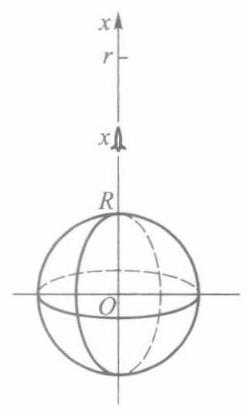
\includegraphics[width=.3\textwidth]{images/P094.jpg}
	\caption{图 $11-1$}
	\label{fig:P094}
\end{figure}

设地球半径为 \(R\) ,火箭质量为 \(m\) ,地面上的重力加速度为 \(g\) . 按万有引力定律,在距地心 \(x\left( { \geq  R}\right)\) 处火箭所受的引力为
\[
F = \frac{{mg}{R}^{2}}{{x}^{2}}.
\]
于是火箭从地面上升到距离地心为 \(r\left( { > R}\right)\) 处需做的功为
\[
{\int }_{R}^{r}\frac{{mg}{R}^{2}}{{x}^{2}}\mathrm{\;d}x = {mg}{R}^{2}\left( {\frac{1}{R} - \frac{1}{r}}\right) .
\]
当 \(r \rightarrow   + \infty\) 时,其极限 \({mgR}\) 就是火箭无限远离地球需做的功. 我们很自然地会把这极限写作上限为 \(+ \infty\) 的“积分”:
\[
{\int }_{R}^{+\infty }\frac{{mg}{R}^{2}}{{x}^{2}}\mathrm{\;d}x = \mathop{\lim }\limits_{{r \rightarrow   + \infty }}{\int }_{R}^{r}\frac{{mg}{R}^{2}}{{x}^{2}}\mathrm{\;d}x = {mgR}.
\]
最后,由机械能守恒定律可求得初速度 \({v}_{0}\) 至少应使
\[
\frac{1}{2}m{v}_{0}^{2} = {mgR}.
\]
用 \(g = {9.81}\mathrm{\;m}/{\mathrm{s}}^{2},R = {6.371} \times  {10}^{6}\mathrm{\;m}\) 代入,便得
\[
{v}_{0} = \sqrt{2gR} \approx  {11.2}\left( {\mathrm{\;{km}}/\mathrm{s}}\right) .
\]
%例 2
\begin{example}

\end{example}
圆柱形桶的内壁高为 \(h\) ,内半径为 \(R\) ,桶底有一半径为 \(r\) 的小孔 (图11-2). 试问从盛满水开始打开小孔直至流完桶中的水,共需多少时间?

从物理学知道, 在不计摩擦力的情形下, 当桶内水位高度为 \(h - x\) 时,水从孔中流出的流速 (单位时间内流过单位截面积的流量) 为
\[
v = \sqrt{{2g}\left( {h - x}\right) },
\]
\begin{figure}
	\centering
	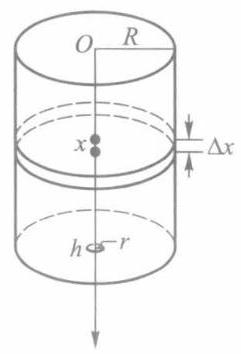
\includegraphics[width=.3\textwidth]{images/P095.jpg}
	\caption{图 $11-2$}
	\label{fig:P095}
\end{figure}

其中 \(g\) 为重力加速度.

设在很小一段时间 \(\mathrm{d}t\) 内,桶中液面降低的微小量为 \(\mathrm{d}x\) ,它们之间应满足
\[
\pi {R}^{2}\mathrm{\;d}x = {v\pi }{r}^{2}\mathrm{\;d}t,
\]
由此则有
\[
\mathrm{d}t = \frac{{R}^{2}}{{r}^{2}\sqrt{{2g}\left( {h - x}\right) }}\mathrm{\;d}x,x \in  \lbrack 0,h).
\]
所以流完一桶水所需时间在形式上亦可写成“积分”:
\[
{t}_{f} = {\int }_{0}^{h}\frac{{R}^{2}}{{r}^{2}\sqrt{{2g}\left( {h - x}\right) }}\mathrm{d}x.
\]
但是在这里因为被积函数是 \(\lbrack 0,h)\) 上的无界函数,所以它的确切含义应该是
\[
{t}_{f} = \mathop{\lim }\limits_{{u \rightarrow  {h}^{ - }}}{\int }_{0}^{u}\frac{{R}^{2}}{{r}^{2}\sqrt{{2g}\left( {h - x}\right) }}\mathrm{d}x
\]
\[
= \mathop{\lim }\limits_{{u \rightarrow  {h}^{ - }}}\sqrt{\frac{2}{g}} \cdot  \frac{{R}^{2}}{{r}^{2}}\left( {\sqrt{h} - \sqrt{h - u}}\right)
\]
\[
= \sqrt{\frac{2h}{g}}{\left( \frac{R}{r}\right) }^{2}\text{ . }
\]
相对于以前所讲的定积分 (不妨称之为正常积分) 而言, 例 1 和例 2 分别提出了两类反常积分.

\subsection{两类反常积分的定义}

%定义  1
\begin{definition}{}{def:}

\end{definition}
设函数 \(f\) 定义在无穷区间 \(\lbrack a, + \infty )\) 上,且在任何有限区间 \(\left\lbrack  {a,u}\right\rbrack\) 上可积. 如果存在极限
\[
\mathop{\lim }\limits_{{u \rightarrow   + \infty }}{\int }_{a}^{u}f\left( x\right) \mathrm{d}x = J, \tag{1}
\]
则称此极限 \(J\) 为函数 \(f\) 在 \(\lbrack a, + \infty )\) 上的无穷限反常积分 (简称无穷积分),记作
\[
J = {\int }_{a}^{+\infty }f\left( x\right) \mathrm{d}x,
\]
 (1')

并称 \({\int }_{a}^{+\infty }f\left( x\right) \mathrm{d}x\) 收敛. 如果极限 (1) 不存在,为方便起见,亦称 \({\int }_{a}^{+\infty }f\left( x\right) \mathrm{d}x\) 发散.

类似地,可定义 \(f\) 在 \(( - \infty ,b\rbrack\) 上的无穷积分:
\[
{\int }_{-\infty }^{b}f\left( x\right) \mathrm{d}x = \mathop{\lim }\limits_{{u \rightarrow   - \infty }}{\int }_{u}^{b}f\left( x\right) \mathrm{d}x. \tag{2}
\]
对于 \(f\) 在 \(\left( {-\infty , + \infty }\right)\) 上的无穷积分,用前面两种无穷积分来定义:
\[
{\int }_{-\infty }^{+\infty }f\left( x\right) \mathrm{d}x = {\int }_{-\infty }^{a}f\left( x\right) \mathrm{d}x + {\int }_{a}^{+\infty }f\left( x\right) \mathrm{d}x, \tag{3}
\]
其中 \(a\) 为任一实数. 当且仅当等号右边两个无穷积分都收敛时,它才是收敛的.

%注
\begin{remark}

\end{remark}
1 无穷积分 (3) 的收敛性与收敛时的值,都和实数 \(a\) 的选取无关.

%注
\begin{remark}

\end{remark}
2 由于无穷积分 (3) 是由 (1)、(2) 两类无穷积分来定义的,因此, \(f\) 在任何有限区间 \(\left\lbrack  {v,u}\right\rbrack   \subset  \left( {-\infty , + \infty }\right)\) 上,首先必须是可积的.

%注
\begin{remark}

\end{remark}
3 \({\int }_{a}^{+\infty }f\left( x\right) \mathrm{d}x\) 收敛的几何意义是: 若 \(f\) 在 \(\lbrack a, + \infty )\) 上为非负连续函数,则图 11-3 中介于曲线 \(y = f\left( x\right)\) ,直线 \(x = a\) 以及 \(x\) 轴之间那一块向右无限延伸的阴影区域有面积 \(J\) .

\begin{figure}
	\centering
	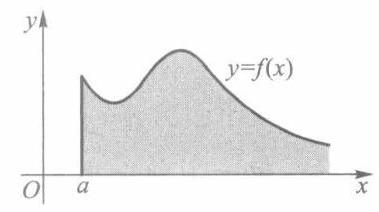
\includegraphics[width=.3\textwidth]{images/P096.jpg}
	\caption{图 $11-3$}
	\label{fig:P096}
\end{figure}

%例 3
\begin{example}

\end{example}
讨论无穷积分
\[
{\int }_{1}^{+\infty }\frac{\mathrm{d}x}{{x}^{p}} \tag{4}
\]
的敛散性.

%解
\begin{solution}

\end{solution}
由于
\[
{\int }_{1}^{u}\frac{\mathrm{d}x}{{x}^{p}} = \left\{  \begin{array}{ll} \frac{1}{1 - p}\left( {{u}^{1 - p} - 1}\right) , & p \neq  1, \\  \ln u, & p = 1, \end{array}\right.
\]
\[
\mathop{\lim }\limits_{{u \rightarrow   + \infty }}{\int }_{1}^{u}\frac{\mathrm{d}x}{{x}^{p}} = \left\{  \begin{array}{ll} \frac{1}{p - 1}, & p > 1, \\   + \infty , & p \leq  1. \end{array}\right.
\]
因此无穷积分 (4) 当 \(p > 1\) 时收敛,其值为 \(\frac{1}{p - 1}\) ; 而当 \(p \leq\) 1 时发散于 \(+ \infty\) .

\begin{figure}
	\centering
	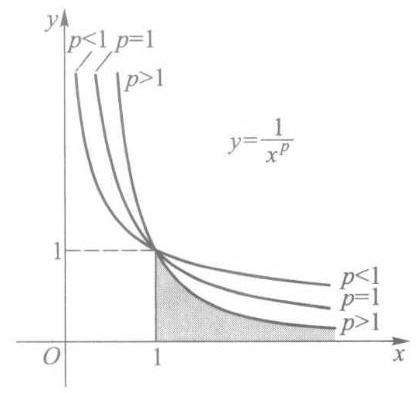
\includegraphics[width=.3\textwidth]{images/P097.jpg}
	\caption{图 $11-4$}
	\label{fig:P097}
\end{figure}

从图 11-4 看到,例 3 的结论是很直观的: \(p\) 的值越大,曲线 \(y = \frac{1}{{x}^{p}}\) 当 \(x > 1\) 时越靠近 \(x\) 轴,从而曲线下方的阴影区域存在有限面积的可能性也就越大.

%例 4
\begin{example}

\end{example}
讨论下列无穷积分的敛散性:

1) \({\int }_{2}^{+\infty }\frac{\mathrm{d}x}{x{\left( \ln x\right) }^{p}}\) ;

2) \({\int }_{-\infty }^{+\infty }\frac{\mathrm{d}x}{1 + {x}^{2}}\) .

%解
\begin{solution}

\end{solution}
1) 由于无穷积分是通过变限定积分的极限来定义的, 因此有关定积分的换元积分法和分部积分法一般都可引用到无穷积分中来. 对于本例来说, 就有
\[
{\int }_{2}^{+\infty }\frac{\mathrm{d}x}{x{\left( \ln x\right) }^{p}} = {\int }_{\ln 2}^{+\infty }\frac{\mathrm{d}t}{{t}^{p}}.
\]
从例 3 知道,该无穷积分当 \(p > 1\) 时收敛,当 \(p \leq  1\) 时发散.

2) 任取实数 \(a\) ,讨论如下两个无穷积分:
\[
{\int }_{-\infty }^{a}\frac{\mathrm{d}x}{1 + {x}^{2}}\text{ 和 }{\int }_{a}^{+\infty }\frac{\mathrm{d}x}{1 + {x}^{2}}.
\]
由于
\[
\mathop{\lim }\limits_{{u \rightarrow   - \infty }}{\int }_{u}^{a}\frac{\mathrm{d}x}{1 + {x}^{2}} = \mathop{\lim }\limits_{{u \rightarrow   - \infty }}\left( {\arctan a - \arctan u}\right)  = \arctan a + \frac{\pi }{2},
\]
\[
\mathop{\lim }\limits_{{v \rightarrow   + \infty }}{\int }_{a}^{v}\frac{\mathrm{d}x}{1 + {x}^{2}} = \mathop{\lim }\limits_{{v \rightarrow   + \infty }}\left( {\arctan v - \arctan a}\right)  = \frac{\pi }{2} - \arctan a,
\]
因此这两个无穷积分都收敛. 由定义 1 ,
\[
{\int }_{-\infty }^{+\infty }\frac{\mathrm{d}x}{1 + {x}^{2}} = {\int }_{-\infty }^{a}\frac{\mathrm{d}x}{1 + {x}^{2}} + {\int }_{a}^{+\infty }\frac{\mathrm{d}x}{1 + {x}^{2}} = \pi .
\]
%注
\begin{remark}

\end{remark}
由于上述结果与 \(a\) 无关,因此若取 \(a = 0\) ,则可使计算过程更简洁些.

%定义  2
\begin{definition}{}{def:}

\end{definition}
设函数 \(f\) 定义在区间 \((a,b\rbrack\) 上,在点 \(a\) 的任一右邻域上无界,但在任何内闭区间 \(\left\lbrack  {u,b}\right\rbrack   \subset  (a,b\rbrack\) 上有界且可积. 如果存在极限
\[
\mathop{\lim }\limits_{{u \rightarrow  {a}^{ + }}}{\int }_{u}^{b}f\left( x\right) \mathrm{d}x = J, \tag{5}
\]
则称此极限为无界函数 \(f\) 在 \((a,b\rbrack\) 上的反常积分,记作
\[
J = {\int }_{a}^{b}f\left( x\right) \mathrm{d}x,
\]
 (5′)

并称反常积分 \({\int }_{a}^{b}f\left( x\right) \mathrm{d}x\) 收敛. 如果极限 (5) 不存在,这时也说反常积分 \({\int }_{a}^{b}f\left( x\right) \mathrm{d}x\) 发散.

在定义 2 中,被积函数 \(f\) 在点 \(a\) 近旁是无界的,这时点 \(a\) 称为 \(f\) 的瑕点,而无界函数反常积分 \({\int }_{a}^{b}f\left( x\right) \mathrm{d}x\) 又称为瑕积分.

类似地,可定义瑕点为 \(b\) 时的瑕积分:
\[
{\int }_{a}^{b}f\left( x\right) \mathrm{d}x = \mathop{\lim }\limits_{{u \rightarrow  {b}^{ - }}}{\int }_{a}^{u}f\left( x\right) \mathrm{d}x.
\]
其中 \(f\) 在 \(\lbrack a,b)\) 有定义,在点 \(b\) 的任一左邻域上无界,但在任何 \(\left\lbrack  {a,u}\right\rbrack   \subset  \lbrack a,b)\) 上可积.

若 \(f\) 的瑕点 \(c \in  \left( {a,b}\right)\) ,则定义瑕积分
\[
{\int }_{a}^{b}f\left( x\right) \mathrm{d}x = {\int }_{a}^{c}f\left( x\right) \mathrm{d}x + {\int }_{c}^{b}f\left( x\right) \mathrm{d}x
\]
\[
= \mathop{\lim }\limits_{{u \rightarrow  {c}^{ - }}}{\int }_{a}^{u}f\left( x\right) \mathrm{d}x + \mathop{\lim }\limits_{{v \rightarrow  {c}^{ + }}}{\int }_{v}^{b}f\left( x\right) \mathrm{d}x. \tag{6}
\]
其中 \(f\) 在 \(\left\lbrack  {a,c) \cup  (c,b}\right\rbrack\) 上有定义,在点 \(c\) 的任一邻域上无界,但在任何 \(\left\lbrack  {a,u}\right\rbrack   \subset  \lbrack a,c)\) 和 \(\left\lbrack  {v,b}\right\rbrack   \subset  (c,b\rbrack\) 上都可积. 当且仅当 (6) 式右边两个瑕积分都收敛时,左边的瑕积分才是收敛的.

又若 \(a,b\) 两点都是 \(f\) 的瑕点,而 \(f\) 在任何 \(\left\lbrack  {u,v}\right\rbrack   \subset  \left( {a,b}\right)\) 上可积,这时定义瑕积分
\[
{\int }_{a}^{b}f\left( x\right) \mathrm{d}x = {\int }_{a}^{c}f\left( x\right) \mathrm{d}x + {\int }_{c}^{b}f\left( x\right) \mathrm{d}x
\]
\[
= \mathop{\lim }\limits_{{u \rightarrow  {a}^{ + }}}{\int }_{u}^{c}f\left( x\right) \mathrm{d}x + \mathop{\lim }\limits_{{v \rightarrow  {b}^{ - }}}{\int }_{c}^{v}f\left( x\right) \mathrm{d}x, \tag{7}
\]
其中 \(c\) 为(a, b)上任一实数. 同样地,当且仅当 (7) 式右边两个瑕积分都收敛时,左边的瑕积分才是收敛的.

%例 5
\begin{example}

\end{example}
计算瑕积分 \({\int }_{0}^{1}\frac{\mathrm{d}x}{\sqrt{1 - {x}^{2}}}\) 的值.

%解
\begin{solution}

\end{solution}
被积函数 \(f\left( x\right)  = \frac{1}{\sqrt{1 - {x}^{2}}}\) 在 \(\lbrack 0,1)\) 上连续,从而在任何 \(\left\lbrack  {0,u}\right\rbrack   \subset  \lbrack 0,1)\) 上可积, \(x = 1\) 为其瑕点. 依定义 2 求得
\[
{\int }_{0}^{1}\frac{\mathrm{d}x}{\sqrt{1 - {x}^{2}}} = \mathop{\lim }\limits_{{u \rightarrow  {1}^{ - }}}{\int }_{0}^{u}\frac{\mathrm{d}x}{\sqrt{1 - {x}^{2}}} = \mathop{\lim }\limits_{{u \rightarrow  {1}^{ - }}}\arcsin u = \frac{\pi }{2}.
\]
%例 6
\begin{example}

\end{example}
讨论瑕积分
\[
{\int }_{0}^{1}\frac{\mathrm{d}x}{{x}^{q}}\left( {q > 0}\right)  \tag{8}
\]
的收敛性.

%解
\begin{solution}

\end{solution}
被积函数在 \((0,1\rbrack\) 上连续, \(x = 0\) 为其瑕点. 由于
\[
{\int }_{u}^{1}\frac{\mathrm{d}x}{{x}^{q}} = \left\{  {\begin{array}{ll} \frac{1}{1 - q}\left( {1 - {u}^{1 - q}}\right) , & q \neq  1, \\   - \ln u, & q = 1 \end{array}\left( {0 < u < 1}\right) ,}\right.
\]
故当 \(0 < q < 1\) 时,瑕积分 (8) 收敛,且
\[
{\int }_{0}^{1}\frac{\mathrm{d}x}{{x}^{q}} = \mathop{\lim }\limits_{{u \rightarrow  {0}^{ + }}}{\int }_{u}^{1}\frac{\mathrm{d}x}{{x}^{q}} = \frac{1}{1 - q};
\]
而当 \(q \geq  1\) 时,瑕积分 (8) 发散于 \(+ \infty\) .

上述结论在图 11-4 中同样能获得直观的反映.

如果把例 3 与例 6 联系起来, 考察反常积分
\[
{\int }_{0}^{+\infty }\frac{\mathrm{d}x}{{x}^{p}}\left( {p > 0}\right) . \tag{9}
\]
我们定义
\[
{\int }_{0}^{+\infty }\frac{\mathrm{d}x}{{x}^{p}} = {\int }_{0}^{1}\frac{\mathrm{d}x}{{x}^{p}} + {\int }_{1}^{+\infty }\frac{\mathrm{d}x}{{x}^{p}},
\]
它当且仅当右边的瑕积分和无穷积分都收敛时才收敛. 但由例 3 与例 6 的结果可知, 这两个反常积分不能同时收敛,故反常积分 (9) 对任何实数 \(p\) 都是发散的.

\subsection{习题 11.1}

1. 讨论下列无穷积分是否收敛? 若收敛, 则求其值:

(1) \({\int }_{0}^{+\infty }x{\mathrm{e}}^{-{x}^{2}}\mathrm{\;d}x\) ;

(2) \({\int }_{-\infty }^{+\infty }x{\mathrm{e}}^{-{x}^{2}}\mathrm{\;d}x\) ；

(3) \({\int }_{0}^{+\infty }\frac{1}{\sqrt{{\mathrm{e}}^{x}}}\mathrm{\;d}x\) ;

(4) \({\int }_{1}^{+\infty }\frac{\mathrm{d}x}{{x}^{2}\left( {1 + x}\right) }\) ;

(5) \({\int }_{-\infty }^{+\infty }\frac{\mathrm{d}x}{4{x}^{2} + {4x} + 5}\) ;

(6) \({\int }_{0}^{+\infty }{\mathrm{e}}^{-x}\sin x\mathrm{\;d}x\) ;

(7) \({\int }_{-\infty }^{+\infty }{\mathrm{e}}^{x}\sin x\mathrm{\;d}x\) ;

(8) \({\int }_{0}^{+\infty }\frac{\mathrm{d}x}{\sqrt{1 + {x}^{2}}}\) .

2. 讨论下列瑕积分是否收敛? 若收敛, 则求其值:

(1) \({\int }_{a}^{b}\frac{\mathrm{d}x}{{\left( x - a\right) }^{p}}\) ;

(2) \({\int }_{0}^{1}\frac{\mathrm{d}x}{1 - {x}^{2}}\) ;

(3) \({\int }_{0}^{2}\frac{\mathrm{d}x}{\sqrt{\left| x - 1\right| }}\) ;

(4) \({\int }_{0}^{1}\frac{x}{\sqrt{1 - {x}^{2}}}\mathrm{\;d}x\) ;

(5) \({\int }_{0}^{1}\ln x\mathrm{\;d}x\) ;

(6) \({\int }_{0}^{1}\sqrt{\frac{x}{1 - x}}\mathrm{\;d}x\) ;

(7) \({\int }_{0}^{1}\frac{\mathrm{d}x}{\sqrt{x - {x}^{2}}}\) ;

(8) \({\int }_{0}^{1}\frac{\mathrm{d}x}{x{\left( \ln x\right) }^{p}}\) .

3. 举例说明: 瑕积分 \({\int }_{a}^{b}f\left( x\right) \mathrm{d}x\) 收敛时, \({\int }_{a}^{b}{f}^{2}\left( x\right) \mathrm{d}x\) 不一定收敛.

4. 举例说明: \({\int }_{a}^{+\infty }f\left( x\right) \mathrm{d}x\) 收敛且 \(f\) 在 \(\lbrack a, + \infty )\) 上连续时,不一定有 \(\mathop{\lim }\limits_{{x \rightarrow   + \infty }}f\left( x\right)  = 0\) .

5. 证明: 若 \({\int }_{a}^{+\infty }f\left( x\right) \mathrm{d}x\) 收敛,且存在极限 \(\mathop{\lim }\limits_{{x \rightarrow   + \infty }}f\left( x\right)  = A\) ,则 \(A = 0\) .

6. 证明: 若 \(f\) 在 \(\lbrack a, + \infty )\) 上可导,且 \({\int }_{a}^{+\infty }f\left( x\right) \mathrm{d}x\) 与 \({\int }_{a}^{+\infty }{f}^{\prime }\left( x\right) \mathrm{d}x\) 都收敛,则 \(\mathop{\lim }\limits_{{x \rightarrow   + \infty }}f\left( x\right)  = 0\) .

\section{无穷积分的性质与敛散判别}

\subsection{无穷积分的性质}

由定义知道,无穷积分 \({\int }_{a}^{+\infty }f\left( x\right) \mathrm{d}x\) 收敛与否,取决于函数 \(F\left( u\right)  = {\int }_{a}^{u}f\left( x\right) \mathrm{d}x\) 在 \(u \rightarrow\)  \(+ \infty\) 时是否存在极限. 因此可由函数极限的柯西准则导出无穷积分收敛的柯西准则.

%定理 11.1
\begin{theorem}{}{the:}

\end{theorem}
 无穷积分 \({\int }_{a}^{+\infty }f\left( x\right) \mathrm{d}x\) 收敛的充要条件是: 任给 \(\varepsilon  > 0\) ,存在 \(G \geq  a\) ,只要 \({u}_{1},{u}_{2} > G\) ,便有
\[
\left| {{\int }_{a}^{{u}_{2}}f\left( x\right) \mathrm{d}x - {\int }_{a}^{{u}_{1}}f\left( x\right) \mathrm{d}x}\right|  = \left| {{\int }_{{u}_{1}}^{{u}_{2}}f\left( x\right) \mathrm{d}x}\right|  < \varepsilon .
\]
此外, 还可根据函数极限的性质与定积分的性质, 导出无穷积分的一些相应性质.

性质 1 若 \({\int }_{a}^{+\infty }{f}_{1}\left( x\right) \mathrm{d}x\) 与 \({\int }_{a}^{+\infty }{f}_{2}\left( x\right) \mathrm{d}x\) 都收敛, \({k}_{1},{k}_{2}\) 为任意常数,则 \({\int }_{a}^{+\infty }\left\lbrack  {{k}_{1}{f}_{1}\left( x\right)  + }\right.\)  \(\left. {{k}_{2}{f}_{2}\left( x\right) }\right\rbrack  \mathrm{d}x\) 也收敛,且
\[
{\int }_{a}^{+\infty }\left\lbrack  {{k}_{1}{f}_{1}\left( x\right)  + {k}_{2}{f}_{2}\left( x\right) }\right\rbrack  \mathrm{d}x = {k}_{1}{\int }_{a}^{+\infty }{f}_{1}\left( x\right) \mathrm{d}x + {k}_{2}{\int }_{a}^{+\infty }{f}_{2}\left( x\right) \mathrm{d}x. \tag{1}
\]
性质 2 若 \(f\) 在任何有限区间 \(\left\lbrack  {a,u}\right\rbrack\) 上可积, \(a < b\) ,则 \({\int }_{a}^{+\infty }f\left( x\right) \mathrm{d}x\) 与 \({\int }_{b}^{+\infty }f\left( x\right) \mathrm{d}x\) 同敛态 (即同时收敛或同时发散), 且有
\[
{\int }_{a}^{+\infty }f\left( x\right) \mathrm{d}x = {\int }_{a}^{b}f\left( x\right) \mathrm{d}x + {\int }_{b}^{+\infty }f\left( x\right) \mathrm{d}x, \tag{2}
\]
其中右边第一项是定积分.

性质 2 相当于定积分的积分区间可加性,由它又可导出 \({\int }_{a}^{+\infty }f\left( x\right) \mathrm{d}x\) 收敛的另一充

要条件: 任给 \(\varepsilon  > 0\) ,存在 \(G \geq  a\) ,当 \(u > G\) 时,总有
\[
\left| {{\int }_{u}^{+\infty }f\left( x\right) \mathrm{d}x}\right|  < \varepsilon .
\]
事实上, 这可由
\[
{\int }_{a}^{+\infty }f\left( x\right) \mathrm{d}x = {\int }_{a}^{u}f\left( x\right) \mathrm{d}x + {\int }_{u}^{+\infty }f\left( x\right) \mathrm{d}x
\]
结合无穷积分的收敛定义而得.

性质 3 若 \(f\) 在任何有限区间 \(\left\lbrack  {a,u}\right\rbrack\) 上可积,且有 \({\int }_{a}^{+\infty }\left| {f\left( x\right) }\right| \mathrm{d}x\) 收敛,则 \({\int }_{a}^{+\infty }f\left( x\right) \mathrm{d}x\) 亦必收敛, 并有
\[
\left| {{\int }_{a}^{+\infty }f\left( x\right) \mathrm{d}x}\right|  \leq  {\int }_{a}^{+\infty }\left| {f\left( x\right) }\right| \mathrm{d}x. \tag{3}
\]
%证
\begin{proof}

\end{proof}
由 \({\int }_{a}^{+\infty }\left| {f\left( x\right) }\right| \mathrm{d}x\) 收敛,根据柯西准则 (必要性),任给 \(\varepsilon  > 0\) ,存在 \(G \geq  a\) ,当 \({u}_{2} > {u}_{1} > G\) 时,总有
\[
\left| {\int }_{{u}_{1}}^{{u}_{2}}\right| f\left( x\right) \left| {\mathrm{d}x}\right|  = {\int }_{{u}_{1}}^{{u}_{2}}\left| {f\left( x\right) }\right| \mathrm{d}x < \varepsilon .
\]
利用定积分的绝对值不等式, 又有
\[
\left| {{\int }_{{u}_{1}}^{{u}_{2}}f\left( x\right) \mathrm{d}x}\right|  \leq  {\int }_{{u}_{1}}^{{u}_{2}}\left| {f\left( x\right) }\right| \mathrm{d}x < \varepsilon .
\]
再由柯西准则 (充分性),证得 \({\int }_{a}^{+\infty }f\left( x\right) \mathrm{d}x\) 收敛.

又因 \(\left| {{\int }_{a}^{u}f\left( x\right) \mathrm{d}x}\right|  \leq  {\int }_{a}^{u}\left| {f\left( x\right) }\right| \mathrm{d}x\left( {u > a}\right)\) ,令 \(u \rightarrow   + \infty\) 取极限,立刻得到不等式 (3).

当 \({\int }_{a}^{+\infty }\left| {f\left( x\right) }\right| \mathrm{d}x\) 收敛时,称 \({\int }_{a}^{+\infty }f\left( x\right) \mathrm{d}x\) 为绝对收敛. 性质 3 指出: 绝对收敛的无穷积分, 它自身也一定收敛. 但是它的逆命题一般不成立, 今后将举例说明收敛的无穷积分不一定绝对收敛.

我们称收敛而不绝对收敛者为条件收敛.

\subsection{非负函数无穷积分的敛散判别法}

首先给出非负函数无穷积分的比较判别法.

设 \(f\) 是定义在 \(\lbrack a, + \infty )\) 上的非负函数,且在任何有限区间 \(\left\lbrack  {a,u}\right\rbrack\) 上可积. 由于 \({\int }_{a}^{u}f\left( x\right) \mathrm{d}x\) 关于上限 \(u\) 是单调递增的,因此 \({\int }_{a}^{+\infty }f\left( x\right) \mathrm{d}x\) 收敛的充要条件是 \({\int }_{a}^{u}f\left( x\right) \mathrm{d}x\) 在 \(\lbrack a, + \infty )\) 上存在上界.根据这一分析,便立即导出下述比较判别法 (请读者自己写出证明).

%定理 11.2
\begin{theorem}{}{the:}

\end{theorem}
 (比较原则) 设定义在 \(\lbrack a, + \infty\) ) 上的两个非负函数 \(f\) 和 \(g\) 都在任何有限区间 \(\left\lbrack  {a,u}\right\rbrack\) 上可积,且满足
\[
f\left( x\right)  \leq  g\left( x\right) ,x \in  \lbrack a, + \infty ),
\]
则当 \({\int }_{a}^{+\infty }g\left( x\right) \mathrm{d}x\) 收敛时, \({\int }_{a}^{+\infty }f\left( x\right) \mathrm{d}x\) 必收敛 (或当 \({\int }_{a}^{+\infty }f\left( x\right) \mathrm{d}x\) 发散时, \({\int }_{a}^{+\infty }g\left( x\right) \mathrm{d}x\) 必发散).

%例 1
\begin{example}

\end{example}
讨论 \({\int }_{0}^{+\infty }\frac{\sin x}{1 + {x}^{2}}\mathrm{\;d}x\) 的敛散性.

%解
\begin{solution}

\end{solution}
由于 \(\left| \frac{\sin x}{1 + {x}^{2}}\right|  \leq  \frac{1}{1 + {x}^{2}},x \in  \lbrack 0, + \infty )\) ,以及 \({\int }_{0}^{+\infty }\frac{\mathrm{d}x}{1 + {x}^{2}} = \frac{\pi }{2}\) 收敛 ( §1 例 4 ), 根据比较原则知 \({\int }_{0}^{+\infty }\frac{\sin x}{1 + {x}^{2}}\mathrm{\;d}x\) 绝对收敛.

上述比较原则的极限形式如下.

推论 1 若 \(f\) 和 \(g\) 都在任何有限区间 \(\left\lbrack  {a,u}\right\rbrack\) 上可积,当 \(x \in  \lbrack a, + \infty )\) 时, \(f\left( x\right)  \geq  0\) , \(g\left( x\right)  > 0\) ,且 \(\mathop{\lim }\limits_{{x \rightarrow   + \infty }}\frac{f\left( x\right) }{g\left( x\right) } = c\) ,则有:

(i) 当 \(0 < c <  + \infty\) 时, \({\int }_{a}^{+\infty }f\left( x\right) \mathrm{d}x\) 与 \({\int }_{a}^{+\infty }g\left( x\right) \mathrm{d}x\) 同敛态;

(ii) 当 \(c = 0\) 时,由 \({\int }_{a}^{+\infty }g\left( x\right) \mathrm{d}x\) 收敛可推知 \({\int }_{a}^{+\infty }f\left( x\right) \mathrm{d}x\) 也收敛;

(iii) 当 \(c =  + \infty\) 时,由 \({\int }_{a}^{+\infty }g\left( x\right) \mathrm{d}x\) 发散可推知 \({\int }_{a}^{+\infty }f\left( x\right) \mathrm{d}x\) 也发散.

特别地,如果选用 \({\int }_{1}^{+\infty }\frac{\mathrm{d}x}{{x}^{p}}\) 作为比较对象,则我们有如下两个推论 (称为柯西判别法).

推论 2 设 \(f\) 定义于 \(\lbrack a, + \infty )\left( {a > 0}\right)\) ,且在任何有限区间 \(\left\lbrack  {a,u}\right\rbrack\) 上可积,则有:

(i) 当 \(0 \leq  f\left( x\right)  \leq  \frac{1}{{x}^{p}},x \in  \lbrack a, + \infty )\) ,且 \(p > 1\) 时, \({\int }_{a}^{+\infty }f\left( x\right) \mathrm{d}x\) 收敛;

(ii) 当 \(f\left( x\right)  \geq  \frac{1}{{x}^{p}},x \in  \lbrack a, + \infty )\) ,且 \(p \leq  1\) 时, \({\int }_{a}^{+\infty }f\left( x\right) \mathrm{d}x\) 发散.

推论 3 设 \(f\) 是定义于 \(\lbrack a, + \infty )\) 上的非负函数,在任何有限区间 \(\left\lbrack  {a,u}\right\rbrack\) 上可积,且
\[
\mathop{\lim }\limits_{{x \rightarrow   + \infty }}{x}^{p}f\left( x\right)  = \lambda .
\]
则有

(i) 当 \(p > 1,0 \leq  \lambda  <  + \infty\) 时, \({\int }_{a}^{+\infty }f\left( x\right) \mathrm{d}x\) 收敛;

(ii) 当 \(p \leq  1,0 < \lambda  \leq   + \infty\) 时, \({\int }_{a}^{+\infty }f\left( x\right) \mathrm{d}x\) 发散.

%例 2
\begin{example}

\end{example}
讨论下列无穷限积分的敛散性:

1) \({\int }_{1}^{+\infty }{x}^{\alpha }{\mathrm{e}}^{-x}\mathrm{\;d}x\) ;

2) \({\int }_{0}^{+\infty }\frac{{x}^{2}}{\sqrt{{x}^{5} + 1}}\mathrm{\;d}x\) .

%解
\begin{solution}

\end{solution}
本例中两个被积函数都是非负的.

1) 由于对任何实数 \(\alpha\) ,都有
\[
\mathop{\lim }\limits_{{x \rightarrow   + \infty }}{x}^{2} \cdot  {x}^{\alpha }{\mathrm{e}}^{-x} = \mathop{\lim }\limits_{{x \rightarrow   + \infty }}\frac{{x}^{\alpha  + 2}}{{\mathrm{e}}^{x}} = 0,
\]
因此根据上述推论 \(3\left( {p = 2,\lambda  = 0}\right)\) ,推知 1) 对任何实数 \(\alpha\) 都是收敛的.

2)由于
\[
\mathop{\lim }\limits_{{x \rightarrow   + \infty }}{x}^{\frac{1}{2}} \cdot  \frac{{x}^{2}}{\sqrt{{x}^{5} + 1}} = 1,
\]
因此根据上述推论 \(3\left( {p = \frac{1}{2},\lambda  = 1}\right)\) ,推知 2) 是发散的.

对于 \({\int }_{-\infty }^{b}f\left( x\right) \mathrm{d}x\) 的比较判别亦可类似地进行.

\subsection{一般无穷积分的敛散判别法}

这里来介绍两个判别一般无穷积分敛散的判别法.

%定理 11.3
\begin{theorem}{}{the:}

\end{theorem}
 (狄利克雷判别法) 若 \(F\left( u\right)  = {\int }_{a}^{u}f\left( x\right) \mathrm{d}x\) 在 \(\lbrack a, + \infty )\) 上有界, \(g\left( x\right)\) 在 \(\lbrack a, + \infty )\) 上当 \(x \rightarrow   + \infty\) 时单调趋于 0,则 \({\int }_{a}^{+\infty }f\left( x\right) g\left( x\right) \mathrm{d}x\) 收敛.

%证
\begin{proof}

\end{proof}
由条件设 \(\left| {{\int }_{a}^{u}f\left( x\right) \mathrm{d}x}\right|  \leq  M,u \in  \lbrack a, + \infty )\) . 任给 \(\varepsilon  > 0\) ,由于 \(\mathop{\lim }\limits_{{x \rightarrow   + \infty }}g\left( x\right)  = 0\) ,因此存在 \(G \geq  a\) ,当 \(x > G\) 时,有
\[
\left| {g\left( x\right) }\right|  < \frac{\varepsilon }{4M}.
\]
又因 \(g\) 为单调函数,利用积分第二中值定理 (定理 9.11) 的推论,对于任何 \({u}_{2} > {u}_{1} >\)  \(G\) ,存在 \(\xi  \in  \left\lbrack  {{u}_{1},{u}_{2}}\right\rbrack\) ,使得
\[
{\int }_{{u}_{1}}^{{u}_{2}}f\left( x\right) g\left( x\right) \mathrm{d}x = g\left( {u}_{1}\right) {\int }_{{u}_{1}}^{\xi }f\left( x\right) \mathrm{d}x + g\left( {u}_{2}\right) {\int }_{\xi }^{{u}_{2}}f\left( x\right) \mathrm{d}x.
\]
于是有
\[
\left| {{\int }_{{u}_{1}}^{{u}_{2}}f\left( x\right) g\left( x\right) \mathrm{d}x}\right|  \leq  \left| {g\left( {u}_{1}\right) }\right|  \cdot  \left| {{\int }_{{u}_{1}}^{\xi }f\left( x\right) \mathrm{d}x}\right|  + \left| {g\left( {u}_{2}\right) }\right|  \cdot  \left| {{\int }_{\xi }^{{u}_{2}}f\left( x\right) \mathrm{d}x}\right|
\]
\[
= \left| {g\left( {u}_{1}\right) }\right|  \cdot  \left| {{\int }_{a}^{\xi }f\left( x\right) \mathrm{d}x - {\int }_{a}^{{u}_{1}}f\left( x\right) \mathrm{d}x}\right|  +
\]
\[
\left| {g\left( {u}_{2}\right) }\right|  \cdot  \left| {{\int }_{a}^{{u}_{2}}f\left( x\right) \mathrm{d}x - {\int }_{a}^{\xi }f\left( x\right) \mathrm{d}x}\right|
\]
\[
< \frac{\varepsilon }{4M} \cdot  {2M} + \frac{\varepsilon }{4M} \cdot  {2M} = \varepsilon .
\]
根据柯西准则,证得 \({\int }_{a}^{+\infty }f\left( x\right) g\left( x\right) \mathrm{d}x\) 收敛.

%定理 11.4
\begin{theorem}{}{the:}

\end{theorem}
 (阿贝尔 (Abel) 判别法) 若 \({\int }_{a}^{+\infty }f\left( x\right) \mathrm{d}x\) 收敛, \(g\left( x\right)\) 在 \(\lbrack a, + \infty )\) 上单调有界,则 \({\int }_{a}^{+\infty }f\left( x\right) g\left( x\right) \mathrm{d}x\) 收敛.

这定理同样可用积分第二中值定理来证明, 但又可利用狄利克雷判别法更方便地获得证明 (留作习题).

%例 3
\begin{example}

\end{example}
讨论 \({\int }_{1}^{+\infty }\frac{\sin x}{{x}^{p}}\mathrm{\;d}x\) 与 \({\int }_{1}^{+\infty }\frac{\cos x}{{x}^{p}}\mathrm{\;d}x\left( {p > 0}\right)\) 的敛散性.

%解
\begin{solution}

\end{solution}
这里只讨论前一个无穷积分, 后者有完全相同的结论. 下面分两种情形来讨论:

(i) 当 \(p > 1\) 时, \({\int }_{1}^{+\infty }\frac{\sin x}{{x}^{p}}\mathrm{\;d}x\) 绝对收敛. 这是因为
\[
\left| \frac{\sin x}{{x}^{p}}\right|  \leq  \frac{1}{{x}^{p}},x \in  \lbrack 1, + \infty ),
\]
而 \({\int }_{1}^{+\infty }\frac{\mathrm{d}x}{{x}^{p}}\) 当 \(p > 1\) 时收敛,故由比较原则推知 \({\int }_{1}^{+\infty }\left| \frac{\sin x}{{x}^{p}}\right| \mathrm{d}x\) 收敛.

(ii) 当 \(0 < p \leq  1\) 时, \({\int }_{1}^{+\infty }\frac{\sin x}{{x}^{p}}\mathrm{\;d}x\) 条件收敛. 这是因为对任意 \(u \geq  1\) ,有 \(\left| {{\int }_{1}^{u}\sin x\mathrm{\;d}x}\right|  =\)  \(\left| {\cos 1 - \cos u}\right|  \leq  2\) ,而 \(\frac{1}{{x}^{p}}\) 当 \(p > 0\) 时单调趋于 \(0\left( {x \rightarrow   + \infty }\right)\) ,故由狄利克雷判别法推知 \({\int }_{1}^{+\infty }\frac{\sin x}{{x}^{p}}\mathrm{\;d}x\) 当 \(p > 0\) 时总是收敛的.

另一方面, 由于
\[
\left| \frac{\sin x}{{x}^{p}}\right|  \geq  \frac{{\sin }^{2}x}{x} = \frac{1}{2x} - \frac{\cos {2x}}{2x},x \in  \lbrack 1, + \infty ),
\]
其中 \({\int }_{1}^{+\infty }\frac{\cos {2x}}{2x}\mathrm{\;d}x = \frac{1}{2}{\int }_{2}^{+\infty }\frac{\cos t}{t}\mathrm{\;d}t\) 满足狄利克雷判别条件,是收敛的. 而 \({\int }_{1}^{+\infty }\frac{\mathrm{d}x}{2x}\) 是发散的,因此当 \(0 < p \leq  1\) 时该无穷积分不是绝对收敛的,所以它是条件收敛的.

%例 4
\begin{example}

\end{example}
证明下列无穷积分都是条件收敛的:
\[
{\int }_{1}^{+\infty }\sin {x}^{2}\mathrm{\;d}x,{\int }_{1}^{+\infty }\cos {x}^{2}\mathrm{\;d}x,{\int }_{1}^{+\infty }x\sin {x}^{4}\mathrm{\;d}x.
\]
%证
\begin{proof}

\end{proof}
前两个无穷积分经换元 \(t = {x}^{2}\) 得到
\[
{\int }_{1}^{+\infty }\sin {x}^{2}\mathrm{\;d}x = {\int }_{1}^{+\infty }\frac{\sin t}{2\sqrt{t}}\mathrm{\;d}t,
\]
\[
{\int }_{1}^{+\infty }\cos {x}^{2}\mathrm{\;d}x = {\int }_{1}^{+\infty }\frac{\cos t}{2\sqrt{t}}\mathrm{\;d}t.
\]
由例 3 知它们是条件收敛的.

对于第三个无穷积分,经换元 \(t = {x}^{2}\) 得
\[
{\int }_{1}^{+\infty }x\sin {x}^{4}\mathrm{\;d}x = \frac{1}{2}{\int }_{1}^{+\infty }\sin {t}^{2}\mathrm{\;d}t,
\]
它也是条件收敛的.

从例 4 中三个无穷积分的收敛性可以看到,当 \(x \rightarrow   + \infty\) 时被积函数即使不趋于零, 甚至是无界的, 无穷积分仍有可能收敛.

%例 5
\begin{example}

\end{example}
若 \(f\left( x\right)\) 在 \(\lbrack a, + \infty )\) 上单调,且 \({\int }_{a}^{+\infty }f\left( x\right) \mathrm{d}x\) 收敛,则当 \(x \rightarrow   + \infty\) 时, \(f\left( x\right)\) 趋于 0 .

%证
\begin{proof}

\end{proof}
如果 \(f\left( x\right)\) 在 \(\lbrack a, + \infty )\) 上单调递增,则或者 \(\mathop{\lim }\limits_{{x \rightarrow   + \infty }}f\left( x\right)  =  + \infty\) ,或者存在实数 \(A\) 使得 \(\mathop{\lim }\limits_{{x \rightarrow   + \infty }}f\left( x\right)  = A\) .

(1)若 \(\mathop{\lim }\limits_{{x \rightarrow   + \infty }}f\left( x\right)  =  + \infty\) ,则存在 \(M > 0\) ,对任何 \(x \geq  M\) ,有 \(f\left( x\right)  > 1\) . 于是对任何 \(u > M\) ,有
\[
{\int }_{a}^{u}f\left( x\right) \mathrm{d}x = {\int }_{a}^{M}f\left( x\right) \mathrm{d}x + {\int }_{M}^{u}f\left( x\right) \mathrm{d}x
\]
\[
\geq  {\int }_{a}^{M}f\left( x\right) \mathrm{d}x + u - M \rightarrow   + \infty \left( {u \rightarrow   + \infty }\right) ,
\]
这与无穷积分 \({\int }_{a}^{+\infty }f\left( x\right) \mathrm{d}x\) 收敛相矛盾.

(2)若 \(\mathop{\lim }\limits_{{x \rightarrow   + \infty }}f\left( x\right)  = A\) 且 \(A > 0\) ,则存在 \(M > 0\) ,对任何 \(x \geq  M\) ,有 \(f\left( x\right)  > \frac{A}{2}\) . 于是对任何 \(u >\)  \(M\) ,有
\[
{\int }_{a}^{u}f\left( x\right) \mathrm{d}x = {\int }_{a}^{M}f\left( x\right) \mathrm{d}x + {\int }_{M}^{u}f\left( x\right) \mathrm{d}x
\]
\[
\geq  {\int }_{a}^{M}f\left( x\right) \mathrm{d}x + \left( {u - M}\right)  \cdot  \frac{A}{2} \rightarrow   + \infty \left( {u \rightarrow   + \infty }\right) ,
\]
这与无穷积分 \({\int }_{a}^{+\infty }f\left( x\right) \mathrm{d}x\) 收敛相矛盾. 若 \(A < 0\) ,类似地也会得到这样的矛盾.

因此 \(\mathop{\lim }\limits_{{x \rightarrow   + \infty }}f\left( x\right)  = 0\) .

当 \(f\left( x\right)\) 在 \(\lbrack a, + \infty )\) 上单调递减时,类似可证.

\subsection{习题 11.2}

1. 证明定理 11.2 及其推论 1 .

2. 设 \(f\) 与 \(g\) 是定义在 \(\lbrack a, + \infty )\) 上的函数,对任何 \(u > a\) ,它们在 \(\left\lbrack  {a,u}\right\rbrack\) 上都可积. 证明: 若 \({\int }_{a}^{+\infty }{f}^{2}\left( x\right) \mathrm{d}x\) 与 \({\int }_{a}^{+\infty }{g}^{2}\left( x\right) \mathrm{d}x\) 收敛,则 \({\int }_{a}^{+\infty }f\left( x\right) g\left( x\right) \mathrm{d}x\) 与 \({\int }_{a}^{+\infty }{\left\lbrack  f\left( x\right)  + g\left( x\right) \right\rbrack  }^{2}\mathrm{\;d}x\) 也都收敛. 3. 设 \(f,g,h\) 是定义在 \(\lbrack a, + \infty )\) 上的三个连续函数,且成立不等式 \(h\left( x\right)  \leq  f\left( x\right)  \leq  g\left( x\right)\) . 证明:

(1) 若 \({\int }_{a}^{+\infty }h\left( x\right) \mathrm{d}x\) 与 \({\int }_{a}^{+\infty }g\left( x\right) \mathrm{d}x\) 都收敛,则 \({\int }_{a}^{+\infty }f\left( x\right) \mathrm{d}x\) 也收敛;

(2)又若 \({\int }_{a}^{+\infty }h\left( x\right) \mathrm{d}x = {\int }_{a}^{+\infty }g\left( x\right) \mathrm{d}x = A\) ,则 \({\int }_{a}^{+\infty }f\left( x\right) \mathrm{d}x = A\) .

4. 讨论下列无穷积分的敛散性:

(1) \({\int }_{0}^{+\infty }\frac{\mathrm{d}x}{\sqrt[3]{{x}^{4} + 1}}\) ;

(2) \({\int }_{1}^{+\infty }\frac{x}{1 - {\mathrm{e}}^{x}}\mathrm{\;d}x\) ;

(3) \({\int }_{0}^{+\infty }\frac{\mathrm{d}x}{1 + \sqrt{x}}\) ;

(4) \({\int }_{1}^{+\infty }\frac{x\arctan x}{1 + {x}^{3}}\mathrm{\;d}x\) ;

(5) \({\int }_{1}^{+\infty }\frac{\ln \left( {1 + x}\right) }{{x}^{n}}\mathrm{\;d}x\) ;

(6) \({\int }_{0}^{+\infty }\frac{{x}^{m}}{1 + {x}^{n}}\mathrm{\;d}x\left( {n,m \geq  0}\right)\) .

5. 讨论下列无穷积分为绝对收敛还是条件收敛:

(1) \({\int }_{1}^{+\infty }\frac{\sin \sqrt{x}}{x}\mathrm{\;d}x\) ;

(2) \({\int }_{0}^{+\infty }\frac{\operatorname{sgn}\left( {\sin x}\right) }{1 + {x}^{2}}\mathrm{\;d}x\) ；

(3) \({\int }_{0}^{+\infty }\frac{\sqrt{x}\cos x}{{100} + x}\mathrm{\;d}x\) ;

(4) \({\int }_{e}^{+\infty }\frac{\ln \left( {\ln x}\right) }{\ln x}\sin x\mathrm{\;d}x\) .

6. 举例说明: \({\int }_{a}^{+\infty }f\left( x\right) \mathrm{d}x\) 收敛时, \({\int }_{a}^{+\infty }{f}^{2}\left( x\right) \mathrm{d}x\) 不一定收敛; \({\int }_{a}^{+\infty }f\left( x\right) \mathrm{d}x\) 绝对收敛时, \({\int }_{a}^{+\infty }{f}^{2}\left( x\right) \mathrm{d}x\) 也不一定收敛.

7. 证明: 若 \({\int }_{a}^{+\infty }f\left( x\right) \mathrm{d}x\) 绝对收敛,且 \(\mathop{\lim }\limits_{{x \rightarrow   + \infty }}f\left( x\right)  = 0\) ,则 \({\int }_{a}^{+\infty }{f}^{2}\left( x\right) \mathrm{d}x\) 必定收敛.

8. 证明: 若 \(f\) 是 \(\lbrack a, + \infty )\) 上的单调函数,且 \({\int }_{a}^{+\infty }f\left( x\right) \mathrm{d}x\) 收敛,则 \(f\left( x\right)  = o\left( \frac{1}{x}\right) ,x \rightarrow   + \infty\) .

9. 证明: 若 \(f\) 在 \(\lbrack a, + \infty )\) 上一致连续,且 \({\int }_{a}^{+\infty }f\left( x\right) \mathrm{d}x\) 收敛,则 \(\mathop{\lim }\limits_{{x \rightarrow   + \infty }}f\left( x\right)  = 0\) .

10. 利用狄利克雷判别法证明阿贝尔判别法.

\section{瑕积分的性质与敛散判别}

类似于无穷积分的柯西收敛准则以及其后的三个性质, 瑕积分同样可由函数极限 \(\mathop{\lim }\limits_{{u \rightarrow  {a}^{ + }}}{\int }_{u}^{b}f\left( x\right) \mathrm{d}x = {\int }_{a}^{b}f\left( x\right) \mathrm{d}x\) 的原意写出相应的命题.

%定理 11.5
\begin{theorem}{}{the:}

\end{theorem}
 瑕积分 \({\int }_{a}^{b}f\left( x\right) \mathrm{d}x\) (瑕点为 \(a\) ) 收敛的充要条件是: 任给 \(\varepsilon  > 0\) ,存在 \(\delta  >\) 0,只要 \({u}_{1},{u}_{2} \in  \left( {a,a + \delta }\right)\) ,总有
\[
\left| {{\int }_{{u}_{1}}^{b}f\left( x\right) \mathrm{d}x - {\int }_{{u}_{2}}^{b}f\left( x\right) \mathrm{d}x}\right|  = \left| {{\int }_{{u}_{1}}^{{u}_{2}}f\left( x\right) \mathrm{d}x}\right|  < \varepsilon .
\]
性质 1 设函数 \({f}_{1}\) 与 \({f}_{2}\) 的瑕点同为 \(x = a,{k}_{1},{k}_{2}\) 为常数,则当瑕积分 \({\int }_{a}^{b}{f}_{1}\left( x\right) \mathrm{d}x\) 与 \({\int }_{a}^{b}{f}_{2}\left( x\right) \mathrm{d}x\) 都收敛时,瑕积分 \({\int }_{a}^{b}\left\lbrack  {{k}_{1}{f}_{1}\left( x\right)  + {k}_{2}{f}_{2}\left( x\right) }\right\rbrack  \mathrm{d}x\) 必定收敛,并有
\[
{\int }_{a}^{b}\left\lbrack  {{k}_{1}{f}_{1}\left( x\right)  + {k}_{2}{f}_{2}\left( x\right) }\right\rbrack  \mathrm{d}x = {k}_{1}{\int }_{a}^{b}{f}_{1}\left( x\right) \mathrm{d}x + {k}_{2}{\int }_{a}^{b}{f}_{2}\left( x\right) \mathrm{d}x. \tag{1}
\]
性质 2 设函数 \(f\) 的瑕点为 \(x = a,c \in  \left( {a,b}\right)\) 为任一常数. 则瑕积分 \({\int }_{a}^{b}f\left( x\right) \mathrm{d}x\) 与 \({\int }_{a}^{c}f\left( x\right) \mathrm{d}x\) 同敛态,并有
\[
{\int }_{a}^{b}f\left( x\right) \mathrm{d}x = {\int }_{a}^{c}f\left( x\right) \mathrm{d}x + {\int }_{c}^{b}f\left( x\right) \mathrm{d}x, \tag{2}
\]
其中 \({\int }_{c}^{b}f\left( x\right) \mathrm{d}x\) 为定积分.

性质 3 设函数 \(f\) 的瑕点为 \(x = a,f\) 在 \((a,b\rbrack\) 的任一内闭区间 \(\left\lbrack  {u,b}\right\rbrack\) 上可积. 则当 \({\int }_{a}^{b}\left| {f\left( x\right) }\right| \mathrm{d}x\) 收敛时, \({\int }_{a}^{b}f\left( x\right) \mathrm{d}x\) 也必定收敛,并有
\[
\left| {{\int }_{a}^{b}f\left( x\right) \mathrm{d}x}\right|  \leq  {\int }_{a}^{b}\left| {f\left( x\right) }\right| \mathrm{d}x. \tag{3}
\]
同样地,当 \({\int }_{a}^{b}\left| {f\left( x\right) }\right| \mathrm{d}x\) 收敛时,称 \({\int }_{a}^{b}f\left( x\right) \mathrm{d}x\) 为绝对收敛. 又称收敛而不绝对收敛的瑕积分是条件收敛的.

判别非负函数瑕积分收敛的比较原则及其推论如下:

%定理 11.6
\begin{theorem}{}{the:}

\end{theorem}
 (比较原则) 设定义在 \((a,b\rbrack\) 上的两个函数 \(f\) 与 \(g\) ,瑕点同为 \(x = a\) ,在任何 \(\left\lbrack  {u,b}\right\rbrack   \subset  (a,b\rbrack\) 上都可积,且满足
\[
0 \leq  f\left( x\right)  \leq  g\left( x\right) ,x \in  (a,b\rbrack .
\]
则当 \({\int }_{a}^{b}g\left( x\right) \mathrm{d}x\) 收敛时, \({\int }_{a}^{b}f\left( x\right) \mathrm{d}x\) 必定收敛 (或者,当 \({\int }_{a}^{b}f\left( x\right) \mathrm{d}x\) 发散时, \({\int }_{a}^{b}g\left( x\right) \mathrm{d}x\) 亦必发散).

推论 1 又若 \(f\left( x\right)  \geq  0,g\left( x\right)  > 0\) ,且 \(\mathop{\lim }\limits_{{x \rightarrow  {a}^{ + }}}\frac{f\left( x\right) }{g\left( x\right) } = c\) ,则有:

(i) 当 \(0 < c <  + \infty\) 时, \({\int }_{a}^{b}f\left( x\right) \mathrm{d}x\) 与 \({\int }_{a}^{b}g\left( x\right) \mathrm{d}x\) 同敛态;

(ii) 当 \(c = 0\) 时,由 \({\int }_{a}^{b}g\left( x\right) \mathrm{d}x\) 收敛可推知 \({\int }_{a}^{b}f\left( x\right) \mathrm{d}x\) 也收敛;

(iii) 当 \(c =  + \infty\) 时,由 \({\int }_{a}^{b}g\left( x\right) \mathrm{d}x\) 发散可推知 \({\int }_{a}^{b}f\left( x\right) \mathrm{d}x\) 也发散.

特别地,如果选用 \({\int }_{a}^{b}\frac{\mathrm{d}x}{{\left( x - a\right) }^{p}}\) 作为比较对象,则我们有如下两个推论 (称为柯西判别法).

推论 2 设 \(f\) 定义在 \((a,b\rbrack\) 上, \(a\) 为其瑕点,且在任何 \(\left\lbrack  {u,b}\right\rbrack   \subset  (a,b\rbrack\) 上可积,则有:

(i) 当 \(0 \leq  f\left( x\right)  \leq  \frac{1}{{\left( x - a\right) }^{p}}\) ,且 \(0 < p < 1\) 时, \({\int }_{a}^{b}f\left( x\right) \mathrm{d}x\) 收敛;

(ii) 当 \(f\left( x\right)  \geq  \frac{1}{{\left( x - a\right) }^{p}}\) ,且 \(p \geq  1\) 时, \({\int }_{a}^{b}f\left( x\right) \mathrm{d}x\) 发散.

推论 3 设 \(f\) 是定义在 \((a,b\rbrack\) 上的非负函数, \(a\) 为其瑕点,且在任何 \(\left\lbrack  {u,b}\right\rbrack   \subset  (a,b\rbrack\) 上可积. 如果
\[
\mathop{\lim }\limits_{{x \rightarrow  {a}^{ + }}}{\left( x - a\right) }^{p}f\left( x\right)  = \lambda ,
\]
则有:

(i) 当 \(0 < p < 1,0 \leq  \lambda  <  + \infty\) 时, \({\int }_{a}^{b}f\left( x\right) \mathrm{d}x\) 收敛;

(ii) 当 \(p \geq  1,0 < \lambda  \leq   + \infty\) 时, \({\int }_{a}^{b}f\left( x\right) \mathrm{d}x\) 发散.

对于一般瑕积分, 也有相应的狄利克雷判别法和阿贝尔判别法.

%定理 11.7
\begin{theorem}{}{the:}

\end{theorem}
 (狄利克雷判别法) 设 \(a\) 为 \(f\left( x\right)\) 的瑕点,函数 \(F\left( u\right)  = {\int }_{a}^{b}f\left( x\right) \mathrm{d}x\) 在 \((a,b\rbrack\) 上有界,函数 \(g\left( x\right)\) 在 \((a,b\rbrack\) 上单调且. \(\mathop{\lim }\limits_{{x \rightarrow  {a}^{ + }}}g\left( x\right)  = 0\) ,则瑕积分 \({\int }_{a}^{b}f\left( x\right) g\left( x\right) \mathrm{d}x\) 收敛.

%定理 11.8
\begin{theorem}{}{the:}

\end{theorem}
(阿贝尔判别法) 设 \(a\) 为 \(f\left( x\right)\) 的瑕点,瑕积分 \({\int }_{a}^{b}f\left( x\right) \mathrm{d}x\) 收敛,函数 \(g\left( x\right)\) 在 \((a,b\rbrack\) 上单调且有界,则瑕积分 \({\int }_{a}^{b}f\left( x\right) g\left( x\right) \mathrm{d}x\) 收敛.

%例 1
\begin{example}

\end{example}
判别下列瑕积分的敛散性:

1) \({\int }_{0}^{1}\frac{\ln x}{\sqrt{x}}\mathrm{\;d}x\) ;

2) \({\int }_{1}^{2}\frac{\sqrt{x}}{\ln x}\mathrm{\;d}x\) .

%解
\begin{solution}

\end{solution}
本例两个瑕积分的被积函数在各自的积分区间上分别保持同号 \(\frac{\ln x}{\sqrt{x}}\) 在 \((0,1\rbrack\) 上恒为负, \(\frac{\sqrt{x}}{\ln x}\) 在 \((1,2\rbrack\) 上恒为正——所以它们的瑕积分收敛与绝对收敛是同一回事.

1) 此瑕积分的瑕点为 \(x = 0\) . 由上述推论 3,当取 \(p = \frac{3}{4} < 1\) 时,有
\[
\lambda  = \mathop{\lim }\limits_{{x \rightarrow  {0}^{ + }}}{x}^{\frac{3}{4}} \cdot  \left| \frac{\ln x}{\sqrt{x}}\right|  =  - \mathop{\lim }\limits_{{x \rightarrow  {0}^{ + }}}\frac{\ln x}{{x}^{-\frac{1}{4}}} = \mathop{\lim }\limits_{{x \rightarrow  {0}^{ + }}}\left( {4{x}^{\frac{1}{4}}}\right)  = 0,
\]
所以瑕积分 1) 收敛.

2) 此瑕积分的瑕点为 \(x = 1\) . 当取 \(p = 1\) 时,由
\[
\lambda  = \mathop{\lim }\limits_{{x \rightarrow  {1}^{ + }}}\left( {x - 1}\right)  \cdot  \frac{\sqrt{x}}{\ln x} = \mathop{\lim }\limits_{{x \rightarrow  {1}^{ + }}}\frac{x - 1}{\ln x} = 1,
\]
推知该瑕积分发散.

最后举一个既是无穷积分又是瑕积分的例子.

%例 2
\begin{example}

\end{example}
讨论反常积分
\[
\Phi \left( \alpha \right)  = {\int }_{0}^{+\infty }\frac{{x}^{\alpha  - 1}}{1 + x}\mathrm{\;d}x
\]
的收敛性.

%解
\begin{solution}

\end{solution}
把反常积分 \(\Phi \left( \alpha \right)\) 写成
\[
\Phi \left( \alpha \right)  = {\int }_{0}^{1}\frac{{x}^{\alpha  - 1}}{1 + x}\mathrm{\;d}x + {\int }_{1}^{+\infty }\frac{{x}^{\alpha  - 1}}{1 + x}\mathrm{\;d}x = I\left( \alpha \right)  + J\left( \alpha \right) .
\]
(i) 先讨论 \(I\left( \alpha \right)\) . 当 \(\alpha  - 1 \geq  0\) ,即 \(\alpha  \geq  1\) 时它是定积分; 当 \(\alpha  < 1\) 时它是瑕积分,瑕点为 \(x = 0\) . 由于
\[
\mathop{\lim }\limits_{{x \rightarrow  {0}^{ + }}}{x}^{1 - \alpha } \cdot  \frac{{x}^{\alpha  - 1}}{1 + x} = 1,
\]
根据定理 11.6 推论 3,当 \(0 < p = 1 - \alpha  < 1\) ,即 \(\alpha  > 0\) 且 \(\lambda  = 1\) 时,瑕积分 \(I\left( \alpha \right)\) 收敛; 当 \(p =\)  \(1 - \alpha  \geq  1\) ,即 \(\alpha  \leq  0\) 且 \(\lambda  = 1\) 时, \(I\left( \alpha \right)\) 发散.

(ii) 再讨论 \(J\left( \alpha \right)\) ,它是无穷积分. 由于
\[
\mathop{\lim }\limits_{{x \rightarrow   + \infty }}{x}^{2 - \alpha } \cdot  \frac{{x}^{\alpha  - 1}}{1 + x} = \mathop{\lim }\limits_{{x \rightarrow   + \infty }}\frac{x}{1 + x} = 1,
\]
根据定理 11.2 推论 3,当 \(p = 2 - \alpha  > 1\) ,即 \(\alpha  < 1\) 且 \(\lambda  = 1\) 时, \(J\left( \alpha \right)\) 收敛; 而当 \(p = 2 - \alpha  \leq  1\) ,即 \(\alpha  \geq  1\) 且 \(\lambda  = 1\) 时, \(J\left( \alpha \right)\) 发散.

综上所述, 把讨论结果列如下表:

\begin{center}
\adjustbox{max width=\textwidth}{
\begin{tabular}{|c|c|c|c|}
\hline
\(\alpha\) & \(\alpha  \leq  0\) & \(0 < \alpha  < 1\) & \(\alpha  \geq  1\) \\
\cline{1-4}
\(I\left( \alpha \right)\) & 发散 & 收敛 & 定积分 \\
\cline{1-4}
\hline
\end{tabular}
}
\end{center}

续表

\begin{center}
\adjustbox{max width=\textwidth}{
\begin{tabular}{|c|c|c|c|}
\hline
\(\alpha\) & \(\alpha  \leq  0\) & \(0 < \alpha  < 1\) & \(\alpha  \geq  1\) \\
\cline{1-4}
\(J\left( \alpha \right)\) & 收敛 & 收敛 & 发散 \\
\cline{1-4}
\(\Phi \left( \alpha \right)\) & 发散 & 收敛 & 发散 \\
\cline{1-4}
\hline
\end{tabular}
}
\end{center}

由此可见,反常积分 \(\Phi \left( \alpha \right)\) 只有当 \(0 < \alpha  < 1\) 时才是收敛的.

\subsection{习题 11.3}

1. 写出性质 3 的证明.

2. 写出定理 11.6 及其推论 1 的证明.

3. 讨论下列瑕积分的敛散性:

(1) \({\int }_{0}^{2}\frac{\mathrm{d}x}{{\left( x - 1\right) }^{2}}\) ;

(2) \({\int }_{0}^{\pi }\frac{\sin x}{{x}^{3/2}}\mathrm{\;d}x\) ；

(3) \({\int }_{0}^{1}\frac{\mathrm{d}x}{\sqrt{x}\ln x}\) ;

(4) \({\int }_{0}^{1}\frac{\ln x}{1 - x}\mathrm{\;d}x\) ;

(5) \({\int }_{0}^{1}\frac{\arctan x}{1 - {x}^{3}}\mathrm{\;d}x\) ;

(6) \({\int }_{0}^{\pi /2}\frac{1 - \cos x}{{x}^{m}}\mathrm{\;d}x\) ;

(7) \({\int }_{0}^{1}\frac{1}{{x}^{\alpha }}\sin \frac{1}{x}\mathrm{\;d}x\) ;

(8) \({\int }_{0}^{+\infty }{\mathrm{e}}^{-x}\ln x\mathrm{\;d}x\) .

4. 计算下列瑕积分的值 (其中 \(n\) 为正整数):

(1) \({\int }_{0}^{1}{\left( \ln x\right) }^{n}\mathrm{\;d}x\) ;

(2) \({\int }_{0}^{1}\frac{{x}^{n}}{\sqrt{1 - x}}\mathrm{\;d}x\) .

5. 证明瑕积分 \(J = {\int }_{0}^{\pi /2}\ln \left( {\sin x}\right) \mathrm{d}x\) 收敛,且 \(J =  - \frac{\pi }{2}\ln 2\) . (提示: 利用 \({\int }_{0}^{\pi /2}\ln \left( {\sin x}\right) \mathrm{d}x =\)  \({\int }_{0}^{\pi /2}\ln \left( {\cos x}\right) \mathrm{d}x\) ,并将它们相加. )

6. 利用上题结果,证明:

(1) \({\int }_{0}^{\pi }\theta \ln \left( {\sin \theta }\right) \mathrm{d}\theta  =  - \frac{{\pi }^{2}}{2}\ln 2\) ;

(2) \({\int }_{0}^{\pi }\frac{\theta \sin \theta }{1 - \cos \theta }\mathrm{d}\theta  = {2\pi }\ln 2\) .

7. 写出定理 11.7 和 11.8 的证明.

\section{第十一章总练习题}

1. 证明下列等式:

(1) \({\int }_{0}^{1}\frac{{x}^{p - 1}}{x + 1}\mathrm{\;d}x = {\int }_{1}^{+\infty }\frac{{x}^{-p}}{x + 1}\mathrm{\;d}x,p > 0\) ;

(2) \({\int }_{0}^{+\infty }\frac{{x}^{p - 1}}{x + 1}\mathrm{\;d}x = {\int }_{0}^{+\infty }\frac{{x}^{-p}}{x + 1}\mathrm{\;d}x,0 < p < 1\) .

2. 证明下列不等式:

(1) \(\frac{\pi }{2\sqrt{2}} < {\int }_{0}^{1}\frac{\mathrm{d}x}{\sqrt{1 - {x}^{4}}} < \frac{\pi }{2}\) ；

(2) \(\frac{1}{2}\left( {1 - \frac{1}{\mathrm{e}}}\right)  < {\int }_{0}^{+\infty }{\mathrm{e}}^{-{x}^{2}}\mathrm{\;d}x < 1 + \frac{1}{2\mathrm{e}}\) .

3. 计算下列反常积分的值:

(1) \({\int }_{0}^{+\infty }{\mathrm{e}}^{-{ax}}\cos {bx}\mathrm{\;d}x\left( {a > 0}\right)\) ;

(2) \({\int }_{0}^{+\infty }{\mathrm{e}}^{-{ax}}\sin {bx}\mathrm{\;d}x\left( {a > 0}\right)\) ；

(3) \({\int }_{0}^{+\infty }\frac{\ln x}{1 + {x}^{2}}\mathrm{\;d}x\) ;

(4) \({\int }_{0}^{\pi /2}\ln \left( {\tan \theta }\right) \mathrm{d}\theta\) .

4. 讨论反常积分 \({\int }_{0}^{+\infty }\frac{\sin {bx}}{{x}^{\lambda }}\mathrm{d}x\left( {b \neq  0}\right) ,\lambda\) 取何值时绝对收敛或条件收敛.

5. 证明: 设 \(f\) 在 \(\lbrack 0, + \infty )\) 上连续, \(0 < a < b\) .

(1) 若 \(\mathop{\lim }\limits_{{x \rightarrow   + \infty }}f\left( x\right)  = k\) ,则
\[
{\int }_{0}^{+\infty }\frac{f\left( {ax}\right)  - f\left( {bx}\right) }{x}\mathrm{\;d}x = \left\lbrack  {f\left( 0\right)  - k}\right\rbrack  \ln \frac{b}{a};
\]
(2)若 \({\int }_{a}^{+\infty }\frac{f\left( x\right) }{x}\mathrm{\;d}x\) 收敛,则
\[
{\int }_{0}^{+\infty }\frac{f\left( {ax}\right)  - f\left( {bx}\right) }{x}\mathrm{\;d}x = f\left( 0\right) \ln \frac{b}{a}.
\]
6. 证明下述命题:

(1) 设 \(f\) 为 \(\lbrack a, + \infty )\) 上的非负连续函数. 若 \({\int }_{a}^{+\infty }{xf}\left( x\right) \mathrm{d}x\) 收敛,则 \({\int }_{a}^{+\infty }f\left( x\right) \mathrm{d}x\) 也收敛.

(2)设 \(f\) 为 \(\lbrack a, + \infty )\) 上的连续可微函数,且当 \(x \rightarrow   + \infty\) 时, \(f\left( x\right)\) 递减地趋于 0,则 \({\int }_{a}^{+\infty }f\left( x\right) \mathrm{d}x\) 收敛的充要条件为 \({\int }_{a}^{+\infty }x{f}^{\prime }\left( x\right) \mathrm{d}x\) 收敛.

7. 设 \(f\left( x\right)\) 在 \(\lbrack 1, + \infty )\) 上二阶连续可微,对于任何 \(x \in  \lbrack 1, + \infty )\) 有 \(f\left( x\right)  > 0\) ,且 \(\mathop{\lim }\limits_{{x \rightarrow   + \infty }}{f}^{\prime \prime }\left( x\right)  =  + \infty\) . 证明: 无穷积分 \({\int }_{1}^{+\infty }\frac{1}{f\left( x\right) }\mathrm{d}x\) 收敛.

\section{第十一章综合自测题}


